\chapter{Two methods for the evolving matrix eigenvalue problem}		\label{Sec:evol_mats}



\section{Introduction}   \label{Subsec:evol_mats-intro}


In this chapter we examine the \textit{evolving matrix eigenvalue problem} in Algorithm \ref{Alg:PGD}, which we define as the \textit{EMEP}, and develop two common eigenvalue methods for handling large-scale eigenvalue problems like the EMEP.  The eigenvalue methods presented in this chapter will allow us to develop new, efficient methods for handling the EMEP in Chapter \ref{Sec:Numerics}.

Section \ref{Subsec:evol_mats-spectral_props} defines the EMEP and examines its evolving spectral structure across matrix iterates $A_k$.  
In particular, we observe that the largest algebraic eigenvalues tend to cluster as the algorithm proceeds, leading to more difficult eigenvalue problems in later matrix iterates.  
To handle these difficult eigenvalue problems, we develop two common eigenvalue methods: the \textit{implicitly restarted Arnoldi method} (IRAM) \cite{sorensen1992implicit} in Section \ref{Subsec:evol_mats-IRAM},
and the \textit{inverse-free preconditioned Krylov subspace method} (EIGIFP) \cite{golub2002inverse} in Section \ref{Subsec:evol_mats-eigifp}.


The IRAM and EIGIFP are based on elementary eigenvalue methods which have inherent strengths and weaknesses related to the spectral structure of the given eigenvalue problem.  
To understand and exploit the theoretical or empirical convergence behavior of the IRAM and EIGIFP, we develop these methods systematically from their elementary eigenvalue methods.









\section{The EMEP: computational costs and spectral properties}		\label{Subsec:evol_mats-spectral_props}

\begin{enumerate}




\item


In this section we define the \textit{evolving matrix eigenvalue problem} (EMEP) and identify the EMEP in Algorithm \ref{Alg:PGD} as the most computationally expensive subroutine in Algorithm \ref{Alg:PGD}.  We see that this EMEP evolves computationally and structurally from early to later iterates in Algorithm \ref{Alg:PGD}.  The high computational cost and changing structure of this EMEP leads us to explore various eigenvalue methods in the remainder of this chapter.


Generally speaking, an EMEP is a sequence of eigenvalue problems in which each eigenvalue problem is dependent on the results of the previous problems.  For each iterate $k$ of the EMEP, we have a Hermitian matrix iterate $A_k \in \caH$ and find its $j$ largest algebraic eigenvalues $\Lambda^{(k)}_j$ and the matrix of corresponding eigenvectors $V^{(k)}_j$.   Next, the previous set of basis matrices $\caV_{k} = \{ V^{(i)}_j \}_{i=0}^{k}$ are used to find the next matrix iterate $A_{k+1}$.  To define the EMEP formally, let $A(\cdot)$ be a function which maps $\caV_{k}$ to $\caH$ for all finite $k \geq 0$ and let $V_0 \in \bbC^{n \times j}$ be an initial basis matrix. Then the EMEP is defined as 
\begin{equation} 		\label{Eqn:EMEP_general}
\begin{array}{ll}
\textnormal{for}
	&	k = 1, 2, \ldots, K		\\
\textnormal{find}	
	&	\left( \Lambda^{(k)}_j, \ V^{(k)}_j \right) \textnormal{ of } A_k
		\\
\textnormal{s.t.}
	&	A_{k} = A(\caV_{k-1})
		\\
	&	\caV_{k-1} = \left\{ V^{(i)}_j \right\}_{i=0}^{k-1}
\end{array}
\end{equation}
where $\Lambda^{(k)}$ are the $j$ largest algebraic eigenvalues of $A_k$ and $V_k$ is the matrix of corresponding eigenvectors.


\


xxx CITE 2 or 3 EMEP examples

\





To see that Algorithm \ref{Alg:PGD} is an EMEP, first note that each eigenvalue problem in Algorithm \ref{Alg:PGD} (steps 2, 6, and 14) requires the $j=2$ largest algebraic eigenvalues of the matrix iterate $A_k = \caA^*y_k$.  (Also note that the EMEP iterate $k$ does not correspond to the Algorithm \ref{Alg:PGD} iterate since step 6 involves a linesearch which may involve more than one eigenvalue problem.)  We will show that each matrix iterate $A_k = \caA^*y_k$ in Algorithm \ref{Alg:PGD} is computed using a variable $y_k$ which is dependent on the previous set of basis vectors $\caV_{k-1} = \{ v_1^{(i)} \}_{i=0}^{k-1}$.  It can be show inductively that $y_k$ is a function of $\caV_{k-1}$.  The initial EMEP iterate $k = 0$ corresponds to the first eigenvalue problem in Algorithm \ref{Alg:PGD}, where $y_0 = \Pi_\caC(b)$ is initialized using the observation vector $b$ and is independent of any eigenvector.  Thus we initialize $v_1^{(0)}$ as the empty set.  If $k >0$ then the update $y_k$ is computed as $y_k = \Pi_{\caC}(y_{k-1}- \alpha_{k-1}  g_{k-1})$, where $g_{k-1} = \caA(v_{k-1} v_{k-1}^*)$ is a function of $v_{k-1}$ and $\alpha_{k-1}$ is determined using a linesearch on the minimization problem
\begin{equation}
\begin{array}{ll}
\min\limits_{\substack{\alpha}}
	&	\lambda_1 \left( \caA^* ( \Pi_\caC ( y_{k-1} - \alpha g_{k-1} ) )  \right).
\end{array}
\end{equation}
Thus $y_k$ is dependent on $v_{k-1}$ and $y_{k-1}$ and Algorithm \ref{Alg:PGD} is an EMEP.



The \textit{Algorithm \ref{Alg:PGD} EMEP} is defined as 
\begin{equation}		\label{Eqn:EMEP_PLGD}
\begin{array}{ll}
\textnormal{for}
	&	k = 1, 2, \ldots, K		\\
\textnormal{find}	
	&	\left( \lambda^{(k)}_1, \ v^{(k)}_1 \right) \textnormal{ and } \left( \lambda^{(k)}_2, \ v^{(k)}_2 \right) \textnormal{ of } A_k
		\\
\textnormal{s.t.}
	&	A_{k} = \caA^*y_k
\end{array}
\end{equation}
where $\lambda^{(k)}_1$ and $\lambda^{(k)}_2$ are the two largest algebraic eigenvalues of the \textit{matrix iterate} $A_k$, and $y_k$ is the previous dual variable generated by Algorithm \ref{Alg:PGD} (from either step 2, 6 or 14).








\item

We many now examine the computational costs of the Algorithm \ref{Alg:PGD} EMEP (\ref{Eqn:EMEP_PLGD}) for PLGD models with Gaussian noise (\ref{Eqn:PhaseLift-GD_Gaussian_noise}).  


As discussed in Section \ref{Subsec:PLGD_algo-algo}, the main computational costs in Algorithm \ref{Alg:PGD} are the EMEP, the primal refinement (step 11), and the dual refinement (step 13).  

The eigenvalue computation for the EMEP is performed using the MATLAB function \texttt{eigs} (described in Section \ref{Subsec:evol_mats-IRAM} for details), and the primal refinement step involves solving (\ref{Eqn:GD-PFD}) using \texttt{minFunc}, a quasi-Newton solver for unstrained optimization, with the descent direction determined using the limited-memory (l-)BFGS method for Hessian approximation \cite{schmidt2005minFunc}.  

Since we are focused on PLGD models with Gaussian noise \ref{Eqn:PhaseLift-GD_Gaussian_noise}, the dual refinement step of Algorithm \ref{Alg:PGD} is skipped (see the end of Section \ref{Subsec:PLGD_term_crit-stagnation} for an explanation).

In both the Algorithm \ref{Alg:PGD} EMEP (\ref{Eqn:EMEP_PLGD}) and the primal refinement step, the primary computational cost comes from $\caA$-products (\ref{Eqn:A_definition_with_masks}), where each $\caA(xx^*)$ product requires $L$ DFTs and each $[\caA^*y]x$ product requires $2L$ DFTs.  Thus we measure computational costs in terms of number of DFTs, following the convention of \cite{DBLP:journals/tit/CandesLS15} and \cite{DBLP:journals/siamsc/FriedlanderM16}.

Also note that the computation of the eigenpair $(\lambda_1, v_1)$ must be very accurate in order to determine an accurate descent step $g = \caA(v_1v_1^*)$ in Algorithm \ref{Alg:PGD}.


Table \ref{Tab:EMEP_costs} depicts the computational costs of Algorithm \ref{Alg:PGD} for a variety of noisy problems.
\begin{table}[H]
\centering
\begin{footnotesize}
\hbox{

\hspace{-0.7cm}
\begin{tabular}{ |ccc|ccc|cc|cc| }
 \hline
			&&&  \multicolumn{3}{c|}{EMEP} 
			&  \multicolumn{2}{c|}{Primal refinement}
			& 	\multicolumn{2}{c|}{All other steps}	\\
$n$ & $L$ & $\epsilon_\text{rel}$ 	& \texttt{eigs} calls  & Minutes & DFTs & Minutes  & DFTs & Minutes  & DFTs   \\
 \hline
 4,096 &  5 & 0.05 & 228 & 13.13  (0.94) &  51,935  (0.97) & 0.73  (0.05) &   1,516  (0.03) & 0.04 &     17 	\\
 4,096 &  5 & 0.15 & 120 & 6.63  (0.94) &  31,085  (0.97) & 0.45  (0.06) &   1,076  (0.03) & 0.01 &     10 \\
 4,096 &  5 & 0.30 &  52 & 3.56  (0.89) &  16,410  (0.95) & 0.45  (0.11) &    854  (0.05) & 0.01 &      4 \\
 4,096 & 10 & 0.05 & 190 & 12.06  (0.96) &  72,587  (0.98) & 0.45  (0.04) &   1,819  (0.02) & 0.03 &     29	\\ 
 4,096 & 10 & 0.15 & 106 & 8.60  (0.96) &  51,450  (0.98) & 0.30  (0.03) &   1,194  (0.02) & 0.02 &     17 \\
 4,096 & 10 & 0.30 & 111 & 17.95  (0.98) & 107,936  (0.99) & 0.36  (0.02) &   1,420  (0.01) & 0.01 &     18 \\
 \hline
16,384 &  5 & 0.05 & 199 & 46.09  (0.95) &  69,745  (0.98) & 2.13  (0.04) &   1,468  (0.02) & 0.06 &     16	\\
16,384 &  5 & 0.15 &  91 & 27.71  (0.95) &  41,880  (0.98) & 1.34  (0.05) &    853  (0.02) & 0.03 &      8	\\
16,384 &  5 & 0.30 &  61 & 30.95  (0.94) &  45,834  (0.98) & 2.04  (0.06) &   1,026  (0.02) & 0.02 &      5	\\
16,384 & 10 & 0.05 & 160 & 56.73  (0.97) &  92,391  (0.98) & 1.64  (0.03) &   1,560  (0.02) & 0.07 &     25	\\
16,384 & 10 & 0.15 & 103 & 36.30  (0.97) &  60,189  (0.98) & 1.21  (0.03) &   1,167  (0.02) & 0.05 &     17	\\
16,384 & 10 & 0.30 &  47 & 18.48  (0.96) &  30,498  (0.98) & 0.65  (0.03) &    617  (0.02) & 0.02 &      8	\\
 \hline
\end{tabular}

}
\end{footnotesize}
\caption{Algorithm \ref{Alg:PGD} runtime and number of DFTs (with percentage of the total in parentheses) for the Algorithm \ref{Alg:PGD} EMEP (\ref{Eqn:EMEP_PLGD}), primal refinement (solving (\ref{Eqn:GD-PFD}) in step 11) and all other operations. Here $n$ is signal size (i.e., number of pixels in the image from Figure \ref{Fig:parrot_signal_iterates}), $L$ is number of observations, and $\epsilon_\textnormal{rel}$ is the noise ratio.} \label{Tab:EMEP_costs}
\end{table}
% experiments.figure.noisyimage_costs


The results in Table \ref{Tab:EMEP_costs} demonstrate the essential computational challenges of Algorithm \ref{Alg:PGD}.  First, the EMEP is the dominant computational cost in the algorithm, and its proportion to other costs (in both runtime and number of DFTs) increases as the size of the model increases.  Additionally, the primal refinement step requires a small but nontrivial amount of computation.  All other operations accounted for $0.00\%$ of the overall runtime. 





\item


Figure \ref{Fig:EMEP_costs_num_mat_vecs} depicts the computational costs the \emep \ for each of the six smaller models from Table \ref{Tab:EMEP_costs}.  For each model, the computational cost of the $k$-th EMEP iterate is measured by the number of matrix-vector products $[\caA^*y_k]x$.

\begin{figure}[H]
\centering
\hbox{\hspace{-1.9cm} 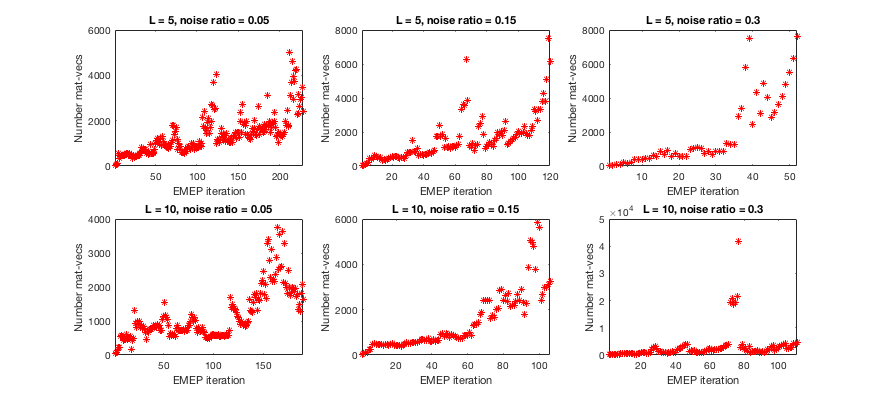
\includegraphics[scale=0.6]{EMEP_costs_num_mat_vecs} }\vspace{-0.4cm}
	\caption{Number of matrix-vector products for each iteration in the \emep for the six smaller models from Table \ref{Tab:EMEP_costs}	.}
\label{Fig:EMEP_costs_num_mat_vecs}
\end{figure}
% experiments.figure.noisyimage_costs

Figure \ref{Fig:EMEP_costs_num_mat_vecs} demonstrates that the computational cost of the \emep \ varies greatly from earlier to later iterates.  In each model, the later iterates account for the majority of the computational cost of the \emep.  





\item

To understand why the computational cost increases as the \emep \ progresses, we must examine the evolving structure of these eigenvalue problems.  In Sections \ref{Subsec:evol_mats-IRAM} and \ref{Subsec:evol_mats-eigifp} we will discuss the impact the spectrum of a matrix has on the (theoretic or empirically expected) convergence rate of various eigenvalue methods.  For now, we will briefly examine how the spectrum varies for the matrix iterates in the \emep.  Figure \ref{Fig:EMEP_full_spectrum} depicts the spectrum of earlier and later iterates for a particular model from Table \ref{Tab:EMEP_costs}.



\begin{figure}[H]
\centering
\hbox{\hspace{-1.9cm} 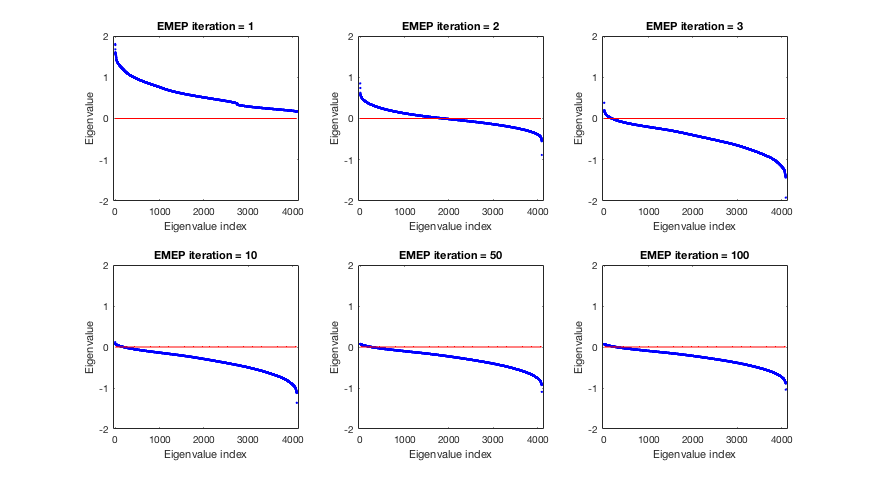
\includegraphics[scale=0.6]{EMEP_full_spectrum} }\vspace{-0.4cm}
	\caption{Spectrum of specific \emep \ matrix iterates $A_k$ for the model from Table \ref{Tab:EMEP_costs} with signal size $n = 4,096$, oversampling $L = 5$, and noise ratio $\epsilon_\text{rel} = 0.15$.}
\label{Fig:EMEP_full_spectrum}
\end{figure}
% experiments.figure.noisyimage_spectrumdist

As we see in Figure \ref{Fig:EMEP_full_spectrum}, the spectrum of the matrix iterates $A_k$ in the \emep \ shifts from completely positive for $A_1$ to mostly negative for later iterates.  This shift in spectrum is a consequence of optimizing the PLGD model (\ref{Eqn:PhaseLift-P-GD}).  The first matrix iterate $A_1 = \caA^*b$ will always be positive-semidefinite because the observations $b_i$ are all nonnegative and thus for all $x$ we have 
\[
x^*[\caA^*b]x 
	= \sum\limits_{\substack{j=1}}^{\substack{L}}
		[FC_jx]^* \textnormal{Diag}(b_j) F C_jx
	\geq 0.
\]
Since Algorithm \ref{Alg:PGD} minimizes the objective function $\lambda_1(\caA^*y_k)$, the largest algebraic eigenvalue $\lambda_1^{(k)}$ of $\caA^*y_k$ can be expected to decrease for later iterates $k$.  


As we will see in Sections \ref{Subsec:evol_mats-IRAM} and \ref{Subsec:evol_mats-eigifp}, the convergence rate of eigenvalue methods often depends on the distance between the desired eigenvalue $\lambda_j$ and the next largest eigenvalue $\lambda_{j+1}$.  Figure \ref{Fig:EMEP_largest_eigvals} depicts the 20 largest algebraic eigenvalues of the \emep \ iterates from Figure \ref{Fig:EMEP_full_spectrum}.


\begin{figure}[H]
\centering
\hbox{\hspace{-1.9cm} 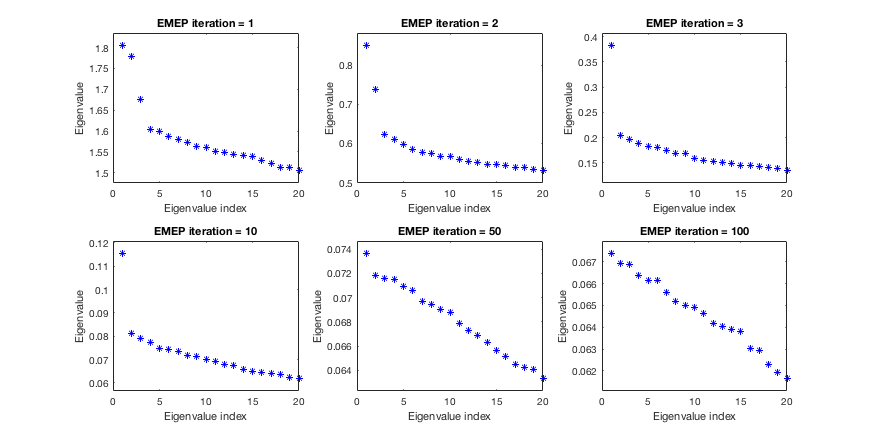
\includegraphics[scale=0.6]{EMEP_largest_eigvals} }\vspace{-0.4cm}
	\caption{Twenty largest algebraic eigenvalues of specific \emep \ matrix iterates $A_k$ for the model from Table \ref{Tab:EMEP_costs} with signal size $n = 4,096$, oversampling $L = 5$, and noise ratio $\epsilon_\text{rel} = 0.15$.}
\label{Fig:EMEP_largest_eigvals}
\end{figure}
% experiments.figure.noisyimage_spectrumdist

Figure \ref{Fig:EMEP_largest_eigvals} demonstrates that the largest algebraic eigenvalues of the matrix iterates $A_k$ cluster together as the \emep \ progresses.  In general, this clustering can be expected.  Section \ref{Subsec:PLGD_algo-algo} established that the PLGD model (\ref{Eqn:PhaseLift-P-GD}) objective function $\lambda_1(\caA^*y)$ is nondifferentiable if the two largest algebraic eigenvalues of $\caA^*y$ are equal.  And Section \ref{Subsec:PLGD_term_crit-stagnation} demonstrated that PLGD models with Gaussian noise (\ref{Eqn:PhaseLift-GD_Gaussian_noise}) typically have nondifferentiable optimal objectives $\lambda_1(\caA^*y_\star)$.  
Thus the two largest algebraic eigenvalues $\lambda_1^{(k)}$ and $\lambda_2^{(k)}$ of the \emep \ can be expected to have a decreasing relative difference
\[
\frac{\lambda_1^{(k)} - \lambda_2^{(k)}}
	{\lambda_1^{(k)}}.
\]






\item


Given the high computational cost of the \emep \ and the evolving structure of this problem, we now proceed to develop a few common methods for handling eigenvalue problems.  The convergence behavior and the strengths and weaknesses of these methods will help us develop more efficient ways of handling the \emep \ in Chapter \ref{Sec:Numerics}. 




\end{enumerate}








\newpage

\section{The implicitly restarted Arnoldi method}		\label{Subsec:evol_mats-IRAM}

\begin{enumerate}


\item

% See following as references:
% http://www.cs.cornell.edu/~bindel/class/cs6210-f09/lec34.pdf
% http://people.inf.ethz.ch/arbenz/ewp/Lnotes/chapter11.pdf
%		Summarizes algorithms, math, convergence criteria, etc.
% ARPACK USERS GUIDE, p 53
%		Algo for IRAM on p 63

% Note: 
%	Prev	Golub
%	p		k, m
%	k		j
%	m		p (= m - j)
%	v		q


In this section we develop the \textit{implicitly restarted Arnoldi method} (IRAM), a common large-scale eigenvalue method which is the default method for handling the \emep.  First proposed by Sorensen \cite{sorensen1992implicit}, \cite{sorensen1997implicitly}, the IRAM is a combination of two essential algorithms.  The \textit{$m$-step Arnoldi iteration} is used to build a matrix $Q_m$ of $m$ basis vectors which approximates the desired eigenspace.  The \textit{$p$-step shifted QR iteration} restarts the matrix $Q_m$ with a specific strategy to damp unwanted eigenvalues, resulting in a smaller matrix $Q_j$ of $j<m$ basis vectors.  Since the $m$-step Arnoldi iteration is an extension of the \textit{power method}, we first discuss the Power method before developing the IRAM.  Altogether, the algorithms in this section are presented in the following order.

\begin{figure}[H] 
\centering
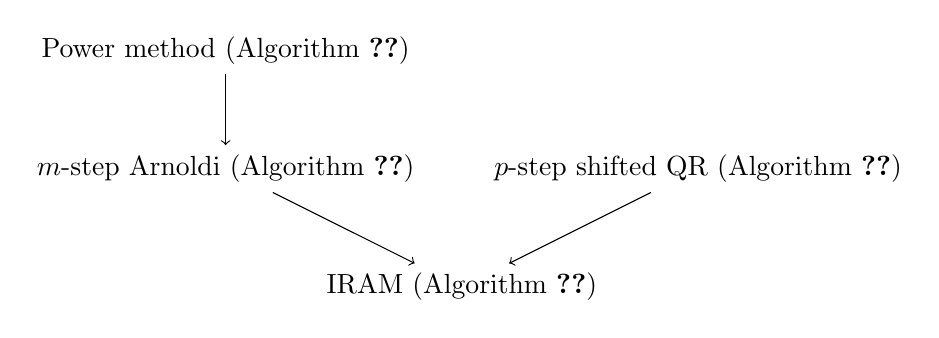
\begin{tikzpicture}
	\node (1) at (0,3) {Power method (Algorithm \ref{Alg:power_method})};
	\node (2) at (0,1.5) {$m$-step Arnoldi (Algorithm \ref{Alg:Arnoldi_iteration})};
	\node (3) at (6,1.5) {$p$-step shifted QR (Algorithm \ref{Alg:shifted_QR_iteration})};
	\node (4) at (3,0) {IRAM (Algorithm \ref{Alg:IRAM})};
	\draw[->] (1) -- (2);
	\draw[->] (2) -- (4);
	\draw[->] (3) -- (4);
\end{tikzpicture}
\caption{Dependency chart for the IRAM.}
\label{Fig:IRAM_flowchart}
\end{figure}

This section follows the treatment found in \cite[Chapters 8, 10]{golub2012matrix}, with occasional minor changes in notation.




\item

The first method we consider is the \textit{power method}, a method for determining the largest magnitude eigenvalue $\lambda_1$ and corresponding eigenvector $v_1$ of a Hermitian matrix $A$.  The power method is based on the property that if $\lambda_1$ is strictly larger in magnitude than the next largest magnitude eigenvalue and the initial vector $q^{(0)}$ has a nonzero component in the direction of $v_1$ (i.e., $v_1^*q^{(0)} \neq 0$), then the sequence
\[
q^{(0)}, \frac{Aq^{(0)}}{||Aq^{(0)}||},  \frac{A^2q^{(0)}}{||A^2q^{(0)}||},  \frac{A^3q^{(0)}}{||A^3q^{(0)}||}, \ldots
\]
will have $v_1$ as its limit.  Formally, the power method is the following algorithm \cite[Section 8.2.1]{golub2012matrix}.


\begin{algorithm}[H]
\caption{Power method}	\label{Alg:power_method}

\begin{algorithmic}[1]
	\Statex 	\textbf{Input:} Hermitian matrix $A$, initial approximate eigenvector $q^{(0)}$, relative tolerance $\textnormal{tol}_\textnormal{rel} > 0$.
	\Statex 	\textbf{Output:} Approximate largest magnitude eigenvalue $\lambda$ and the corresponding eigenvector $v$.
	\State		\textit{Initialize:} $q^{(0)} = q^{(0)}/||q^{(0)}||$, $\rho^{(0)} = [q^{(0)}]^*Aq^{(0)}$, $r^{(0)} = Au^{(0)} - \rho^{(0)}q^{(0)}$, $i= 1$.
	\While {\textit{not converged:} $ ||r^{(i)} || / (||Aq^{(i)}|| + |\rho^{(i)}|) > \textnormal{tol}_\textnormal{rel} $}
		\State		$z^{(i)} = Aq^{(i-1)}$
		\State		$q^{(i)} = z^{(i)} / ||z^{(i)}||$
		\State		$\rho^{(i)} = [q^{(i)}]^* z^{(i)}$
		\State		$r^{(i)} = Aq^{(i)} - \rho^{(i)}q^{(i)}$, $i = i + 1$
	\EndWhile
	\State		\textit{Return:} $(\lambda, v) = (\rho^{(i-1)} , q^{(i-1)})$.
\end{algorithmic}

\end{algorithm}


The simplicity of power method allows for elegant, insightful convergence results like the following theorem, in which we assume the matrix $A$ is real for clarity.

\begin{theorem}			\label{Thm:power_method_conv_rate}
Suppose $A \in \bbR^{n \times n}$ is symmetric with an eigenvalue decomposition
\[
V^*AV = \text{Diag}(\lambda_1, \lambda_2, \ldots, \lambda_n),
\]
where $V = [\ v_1 \ | \ v_2 \ | \cdots | \ v_n \ ]$ is orthogonal and $|\lambda_1| > |\lambda_2| \geq \cdots \geq |\lambda_n|$.  Let the vectors $q^{(i)}$ be generated by Algorithm \ref{Alg:power_method} and define $\theta_i \in [0, \pi/2]$ as 
\[
	\cos(\theta_i) = \left| v_1^Tq^{(i)} \right|.
\]
If $\cos(\theta_0) \neq 0$, then for $i = 0, 1, \ldots$ we have 
\begin{equation} 		\label{Eqn:power_method_conv_rate_1}
\left| \sin(\theta_i) \right| \leq \tan(\theta_0) \left| \frac{\lambda_2}{\lambda_1} \right|^i,
\end{equation}
\begin{equation} 		\label{Eqn:power_method_conv_rate_2}
\left| \lambda^{(i)} - \lambda_1 \right| \leq \max_{2 \leq j \leq n} \left| \lambda_1 - \lambda_i \right| \tan(\theta_0)^2 \left| \frac{\lambda_2}{\lambda_1} \right|^{2i}.
\end{equation}
\end{theorem}

\begin{proof}
See \cite[Theorem 8.2.1]{golub2012matrix}.
\end{proof}

Theorem \ref{Thm:power_method_conv_rate} establishes that the convergence rate of the power method (Algorithm \ref{Alg:power_method}) is dependent on the distance between $|\lambda_1|$ and $|\lambda_2|$.  If this distance $\epsilon = |\lambda_1| - |\lambda_2|$ is very small relative to $|\lambda_1|$, then we have
\[
\left| \frac{\lambda_2}{\lambda_1} \right| = \frac{|\lambda_1| - \epsilon}{|\lambda_1|} = 1 - \frac{\epsilon}{|\lambda_1|} \approx 1,
\]
and $|\sin(\theta_i)|$ in (\ref{Eqn:power_method_conv_rate_1}) may decreases very slowly.  




\item



The next method we consider is the \textit{$m$-step Arnoldi iteration} which extends the power method (Algorithm \ref{Alg:power_method}) to achieve a superior convergence rate.  An iteration of the power method generates a new approximate eigenvector ($q^{(i)}$ from steps 3 and 4) by normalizing the matrix-vector product of the previous vector.  In essence, the power method searches for the largest magnitude eigenvalue $\lambda_1$ and corresponding eigenvector $v_1$ of a matrix $A$ in the one-dimensional subspace $V = \textnormal{span} \{ Aq_1 \}$.  The $m$-step Arnoldi iteration extends the power method by searching for the Ritz pair (\ref{Def:Ritz_pair_val_vec}) ($\theta_1, u_1$) for $A$ with respect to the $m$-dimensional \textit{Krylov subspace}
\begin{equation}
\caK_m(A, q_1) = \textnormal{span}\{ q_1, Aq_1, A^2q_1, \ldots, A^{m-1}q_1 \}.
\label{Def:krylov_subspace}
\end{equation}
Algorithm \ref{Alg:Arnoldi_iteration} (as described in \cite[Algorithm 10.5.1]{golub2012matrix}) builds a unitary basis $Q_m$ of $\caK_m(A, q_1)$ which may be used to find the Ritz pair ($\theta_1, u_1$).
\begin{algorithm}[H]
\caption{$m$-step Arnoldi iteration}	\label{Alg:Arnoldi_iteration}

\begin{algorithmic}[1]
	\Statex		\textbf{Input:} Matrix $A \in \bbC^{n \times n}$, number of Arnoldi steps $m$, initial approximate eigenvector $q_1$.
	\Statex 	\textbf{Output:} Hessenberg matrix $H_m$, basis $Q_m$, residual $r_m$.
	\State		\textit{Initialize:} $q_1  = q_1 / ||q_1||$, \ \ $z = Aq_1$, \ \ $\alpha_1 = q_1^*z$, \ \ $r_1 = z - \alpha_1 q_1$, \ \ $Q_1 = [q_1]$, \ \ $H_1 = [\alpha_1]$.
	\For 			{$i = 1, \ldots, m-1$}
		\State	$\beta_i = ||r_i||$, \ \ $q_{i+1} = r_i / \beta_i$.
		\State	$Q_{i+1} = [Q_i \ | \ q_{i+1}]$, \ \ $\hat{H}_i = \begin{bmatrix}	H_i \\  \beta_i e_i^T	\end{bmatrix}$.
		\State	$z = Aq_{i+1}$.
		\State	$h = Q_{i+1}^*z$, \ \  $r_{i+1} = z - Q_{i+1}h$.
		\State	$H_{i+1} = [\hat{H}_i \ | \ h]$.
	\EndFor
	\State		\textit{Return:} $H_m, Q_m, r_m$.
\end{algorithmic}

\end{algorithm}

In order to obtain a Ritz pair ($\theta, u$) for $A$ with respect to $\caK_m(A, q_1)$, the $m$-step Arnoldi iteration generates an \textit{$m$-step Arnoldi decomposition}
\begin{equation} 		\label{Eqn:Arnoldi_decomp}
AQ_m = Q_m H_m + r_m e_m^*,
\end{equation}
where $H_m$ is an upper Hessenberg matrix.  If $(\theta, w)$ is an eigenpair for $H_m$ and $u = Q_mw$ then (\ref{Eqn:Arnoldi_decomp}) implies
\begin{equation} 			\label{Eqn:Arnoldi_decomp_Ritz_pairs}
(AQ_m - Q_mH_m)w = (A-\theta I) u = (e_m^*w)r_m.
\end{equation}
Additionally, steps 5 and 6 of Algorithm \ref{Alg:Arnoldi_iteration} indicate that $r_m$ is orthogonal to $\caK_m(A, q_1)$, and thus ($\theta, u$) is a Ritz pair for $A$ with respect to $\caK_m(A, q_1)$.  


The use of $\caK_m(A, q_1)$ in Algorithm \ref{Alg:Arnoldi_iteration} allows for superior convergence to Algorithm \ref{Alg:power_method}.  Note that the largest magnitude Ritz pair $(\theta_1, u_1)$ for $A$ with respect to $\caK_m(A, q_1)$ generated by Algorithm \ref{Alg:Arnoldi_iteration}  is guaranteed to be at least comparable to the $m$-th iterate of Algorithm \ref{Alg:power_method} since $A^{m-1}q_1 \in  \caK_m(A, q_1)$.  To compare the convergence rates of Algorithms \ref{Alg:power_method} and \ref{Alg:Arnoldi_iteration} more precisely, assume the matrix $A$ in real and symmetric.  Then the matrix $H_m$ returned by Algorithm \ref{Alg:Arnoldi_iteration} is tridiagonal and this algorithm is equivalent to the \textit{$m$-step Lanczos iteration} \cite[Algorithm 10.1.1]{golub2012matrix}.  In this case, we have the following theorem.  Note that this theorem involves \textit{Chebyshev polynomials} \cite[Section 4.4]{saad2011numerical}, a sequence of polynomials defined recursively as
\begin{equation} 			\label{Def:Chebyshev_polys}
c_k(x) = 2x c_{k-1}(x) - c_{k-2}(x)
\end{equation}
for $k \geq 2$, with $c_0 = 1$ and $c_2 = x$ .

\begin{theorem}   		\label{Thm:Lanczos_conv_rate}
Let $A \in \bbR^{n \times n}$ be symmetric with an eigenvalue decomposition
\[
V^*AV = \text{Diag}(\lambda_1, \lambda_2, \ldots, \lambda_n),
\]
where $V = [\ v_1 \ | \ v_2 \ | \cdots | \ v_n \ ]$ is orthogonal and $\lambda_1 \geq \lambda_2 \geq \cdots \geq \lambda_n$.  Suppose the $m$-step Arnoldi iteration (Algorithm \ref{Alg:Arnoldi_iteration}) is performed and $H_k$ is the tridiagonal matrix returned by this algorithm.  If $\theta_1$ is the largest algebraic eigenvalue of $H_m$, then
\begin{equation} 			\label{Eqn:Lanczos_thm_1}
\lambda_1 \geq \theta_1 \geq \lambda_1 - (\lambda_1 - \lambda_n) 
\left( \frac{\tan(\phi_1)}{c_{m-1}(1+2\rho_1)} \right)^2,
\end{equation}
where $\cos(\phi_1) = |q_1^Tv_1|$,
\begin{equation}		\label{Eqn:Lanczos_thm_2}
\rho_1 = \frac{\lambda_1 - \lambda_2}{\lambda_2 - \lambda_n},
\end{equation}
and $c_{m-1}(x)$ is the Chebyshev polynomial of degree $m-1$.
\end{theorem}

\begin{proof}
See \cite[Theorem 10.1.2]{golub2012matrix}.
\end{proof}

The convergence rate established in Theorem \ref{Thm:Lanczos_conv_rate} may also be applied to Algorithm \ref{Alg:power_method}, giving the following corollary.

\begin{corollary} 			\label{Cor:Lanczos_cor_for_power_method}
Let $A \in \bbR^{n \times n}$ be symmetric and positive semidefinite with an eigenvalue decomposition
\[
V^*AV = \text{Diag}(\lambda_1, \lambda_2, \ldots, \lambda_n),
\]
where $V = [\ v_1 \ | \ v_2 \ | \cdots | \ v_n \ ]$ is orthogonal and $\lambda_1 \geq \lambda_2 \geq \cdots \geq \lambda_n \geq 0$.  Suppose $m$ steps of the power method (Algorithm \ref{Alg:power_method}) are performed and $\gamma_1 = \rho^{(m)}$ is the returned Ritz value.  Then
\begin{equation} 			\label{Eqn:Lanczos_cor_for_power_method}
\lambda_1 \geq \gamma_1 \geq \lambda_1 - (\lambda_1 - \lambda_n) 
\tan^2(\phi_1) \left( \frac{\lambda_2}{\lambda_1} \right)^{2(m-1)},
\end{equation}
where $\cos(\phi_1) = |q_1^Tv_1|$.
\end{corollary}

\begin{proof}
See \cite[Theorem 10.1.2]{golub2012matrix} and replace the Chebyshev polynomial in this proof with $p(x) = x^{k-1}$.
\end{proof}


The lower bounds in Theorem \ref{Thm:Lanczos_conv_rate} and Corollary \ref{Cor:Lanczos_cor_for_power_method} may be used to compare the expected convergence rates for Algorithms \ref{Alg:power_method} and \ref{Alg:Arnoldi_iteration}.  The following comparison is based on \cite[Section 10.1.6]{golub2012matrix}.  Assume $A \in \bbR^{n \times n}$ is symmetric and also positive semidefinite for clarity.  Assume Algorithms \ref{Alg:power_method} and \ref{Alg:Arnoldi_iteration} have been run for $m$ steps with the same initial vector $q_1$.  Let $\gamma_1 = \rho^{(m)}$ be the Ritz value for $A$ generated by step 5 of Algorithm \ref{Alg:power_method}.  And let $\theta_1$ be the Ritz value for $A$ with respect to $\caK_m(A, q_1)$ generated by the largest algebraic eigenvalue of $H_m$ from Algorithm \ref{Alg:Arnoldi_iteration}.  Then we may compare the lower bounds (\ref{Eqn:Lanczos_cor_for_power_method}) for $\gamma_1$ and (\ref{Eqn:Lanczos_thm_1}) for $\theta_1$ by comparing the values
\begin{equation} 		\label{Eqn:power_method_lower_bound}
P_{m-1} = \left( \frac{\lambda_2}{\lambda_1} \right)^{2(m-1)},
\end{equation}
\begin{equation}  	\label{Eqn:Lanczos_lower_bound}
L_{m-1} 
	= \frac{1}{\left[c_{m-1}\left(2\frac{\lambda_1}{\lambda_2} -1 \right)\right]^2} 
	\geq 	\frac{1}{\left[ c_{m-1}\left( 1 + 2 \rho_1 \right) \right]^2}.
\end{equation}
Table \ref{Tab:Lanczos_vs_power_method} compares $P_{m-1}$ and $L_{m-1}$ for a few values of $m$ and $\lambda_1/\lambda_2$.

\begin{table}[H]
\centering
\begin{tabular}{ |c|cc|cc| }
 \hline

 	&	\multicolumn{2}{c|}{$m = 10$}
 		&	\multicolumn{2}{c|}{$m = 20$}	\\
 $\lambda_1 / \lambda_2$	&	$P_{m-1}$	&	$L_{m-1}$
 		&	$P_{m-1}$	&	$L_{m-1}$		\\ 			
 \hline
$1.10$
	&	$1.8 \times 10^{-1}$ & $5.5 \times 10^{-5}$
		&	$2.7 \times 10^{-2}$ & $2.1 \times 10^{-10}$	\\
$1.01$
	&	$8.4 \times 10^{-1}$ & $1.0 \times 10^{-1}$
		&	$6.9 \times 10^{-1}$ & $2.0 \times 10^{-3}$	\\
 \hline
\end{tabular}
\caption{Lower bound terms (\ref{Eqn:power_method_lower_bound}) and (\ref{Eqn:Lanczos_lower_bound}) for Ritz values generated by Algorithms \ref{Alg:power_method} and \ref{Alg:Arnoldi_iteration} } \label{Tab:Lanczos_vs_power_method}
\end{table}

Table \ref{Tab:Lanczos_vs_power_method} demonstrates that the use of the Krylov subspace (\ref{Def:krylov_subspace}) in Algorithm \ref{Alg:Arnoldi_iteration} allows for superior convergence to Algorithm \ref{Alg:power_method}.  Yet this superior convergence rate is slowed somewhat when the desired eigenvalue $\lambda_1$ is close to $\lambda_2$.  For eigenvalue problems where the value $\lambda_1 / \lambda_2$ is very small (like later iterates of the \emep, as demonstrated in Figure \ref{Fig:EMEP_largest_eigvals}), we may seek to increase the number of steps $m$ in Algorithm \ref{Alg:Arnoldi_iteration}.  Yet increasing $m$ can be computationally prohibitive if the eigenvalue problem is very large, requiring significant memory to store $Q_m$ and significant computation to compute the eigenvalue decomposition of $H_m$.




\item

To take advantage of the convergence rate of Algorithm \ref{Alg:Arnoldi_iteration} for larger eigenvalue problems, the Arnoldi decomposition (\ref{Eqn:Arnoldi_decomp}) may be restarted with the \textit{$p$-step shifted QR iteration} developed by \cite{sorensen1992implicit} and discussed in \cite[Sections 10.5.2-3]{golub2012matrix}.  To develop this algorithm, assume we are seeking the $j$ largest eigenvalues of a Hermitian matrix $A \in \bbC^{n \times n}$ and we require that the $m$-step Arnoldi decomposition (\ref{Eqn:Arnoldi_decomp}) $AQ_m = Q_m H_m + r_m e_m^*$ has a fixed size $m > j$.  First we run Algorithm \ref{Alg:Arnoldi_iteration} with the initial vector $q_1$ to obtain $AQ_m = Q_m H_m + r_m e_m^*$.  Next, recall that the matrix $H_m$ may be used to identify the desired Ritz pairs $\{(\theta_i, u_i)\}_{i=1}^j$ for $A$ with respect to $\caK_m(A, q_1)$, as described in (\ref{Eqn:Arnoldi_decomp_Ritz_pairs}).  Yet $H_m$ also contains Ritz values $\theta_{j+1}, \ldots, \theta_m$ which correspond to unwanted eigenvalues of $A$.  To damp these unwanted Ritz values, we may select an appropriate degree $p = m-j$ filter polynomial $p(\lambda)$.  The $p$-step shifted QR iteration uses the filter polynomial
\begin{equation} 			\label{Eqn:filter_poly}
p(\lambda) = c \cdot (\lambda - \mu_1) (\lambda - \mu_2) \cdots (\lambda - \mu_p),
\end{equation}
where $c$ is a constant and the shift values $\mu_1 = \theta_{j+1}, \ldots, \mu_p = \theta_m$ are the $p$ unwanted Ritz values of $A$ with respect to $\caK_m(A, q_1)$.  Algorithm \ref{Alg:shifted_QR_iteration} (as described in \cite[Section 10.5.3]{golub2012matrix}) uses the filter polynomial (\ref{Eqn:filter_poly}) implicitly by applying $p$ shifted QR steps to $H_m$.
%(see \cite[Section 5.2]{golub2012matrix} for details regarding the QR factorization)
\begin{algorithm}[H]
\caption{$p$-step shifted QR iteration (implicit polynomial filtering)}	\label{Alg:shifted_QR_iteration}

\begin{algorithmic}[1]
	\Statex 	\textbf{Input:} Hessenberg matrix $H_m \in \bbC^{m \times m}$ and shift values $\mu_1, \ldots, \mu_p$.
	\Statex 	\textbf{Output:} Processed Hessenberg matrix $H_m^+ \in \bbC^{m \times m}$ and change of basis $V \in \bbC^{m \times m}$, with $H_m^+ = V^*H_mV$.
	\State		Set $H^{(0)} = H_m$.
	\For {$i = 1, \ldots, p$ }
		\State		\textit{QR factorization:} $H^{(i-1)} - \mu_i I = V_iR_i$.
		\State		\textit{Update:} $H^{(i)} = R_iV_i + \mu_iI$.
	\EndFor
	\State		Set $H_m^+ = H^{(p)}$, $V = V_1  V_2 \cdots V_p$.
	\State		\textit{Return:} $H_m^+, V$.
\end{algorithmic}

\end{algorithm}

The following proposition establishes that Algorithm \ref{Alg:shifted_QR_iteration} implicitly applies the filter polynomial $p(\lambda)$ from (\ref{Eqn:filter_poly}) to the initial vector $q_1$ used to create the $m$-step Arnoldi decomposition (\ref{Eqn:Arnoldi_decomp}).

\begin{prop}
Let $A \in \bbC^{n \times n}$ be Hermitian and $AQ_m = Q_mH_m + r_me_m^*$ be the $m$-step Arnoldi decomposition (\ref{Eqn:Arnoldi_decomp}) returned by Algorithm \ref{Alg:Arnoldi_iteration} with initial vector $q_1$.  And let $\mu_1, \ldots, \mu_p$ be the $p$ smallest algebraic eigenvalues of $H_m$.  Run Algorithm \ref{Alg:shifted_QR_iteration} with $H_m$ and $\mu_1, \ldots, \mu_p$ as inputs, and return $H_m^+$, $V = V_1 \cdots V_p$, and $R = R_p \cdots R_1$.

Then the restarted matrix $Q_+ = Q_mV$ will have the first column
\[
q_+ = Q_mV(:,1) = p(A)q_1,
\]
where $p(\lambda)$ is the filter polynomial (\ref{Eqn:filter_poly}) with constant $c = 1/R(1,1)$.
\end{prop}

\begin{proof}
First we must show that 
\begin{equation} 		\label{Eqn:filter_poly_proposition-VR}
VR = (H_m - \mu_1I) \cdots (H_m - \mu_pI).
\end{equation}

Using induction, we see that if $p=1$ then clearly (\ref{Eqn:filter_poly_proposition-VR}) holds.  If $p>1$, then let $\tilde{V}=V_1 \cdots V_{p-1}$ and $\tilde{R} = R_{p-1} \cdots R_1$, and note that $H^{(p-1)} = \tilde{V}^*H_m\tilde{V}$.  Then we have
\[
\begin{split}
VR & = \tilde{V}(V_pR_p)\tilde{R} 
	= \tilde{V} \left( H^{(p-1)} - \mu_pI \right) \tilde{R}
	= \tilde{V}\left( \tilde{V}^*H_m \tilde{V} - \mu_p I \right)\tilde{R}	\\
	& = \left(H_m - \mu_p I \right) \tilde{V}\tilde{R}
	= (H_m - \mu_p I) (H_m - \mu_1 I) \cdots (H_m - \mu_{p-1}I) 	\\
	&=  (H_m - \mu_1I) \cdots (H_m - \mu_pI),
\end{split}
\]
and (\ref{Eqn:filter_poly_proposition-VR}) holds.

Next, note that if the $m$-step Arnoldi decomposition (\ref{Eqn:Arnoldi_decomp}) is right-multiplied by $e_1$, then for all $\mu$ we have
\begin{equation} 			\label{Eqn:filter_poly_propostion-flip}
\left(A - \mu I \right)Q_me_1 = Q_m \left(H_m - \mu I \right) e_1.
\end{equation}

Then we have
\[
\begin{split}
q_+ 
	& = Q_mV(:,1) = Q_m \left[ \frac{1}{R(1,1)}VR e_1 \right] 	\\
	& 	= Q_m p(H_m) e_1 = p(A)Q_m e_1	\\
	& 	= p(A) q_1,
\end{split}
\]
where the third equality is given by (\ref{Eqn:filter_poly_proposition-VR}) and the fourth is given by (\ref{Eqn:filter_poly_propostion-flip}).
\end{proof}


After performing Algorithm \ref{Alg:shifted_QR_iteration}, we have the transformed $m$-step Arnoldi decomposition (\ref{Eqn:Arnoldi_decomp})
\begin{equation}			\label{Eqn:Arnoldi_decomp_transf_shifted_QR}
AQ_+ = Q_+H_+ + r_me_m^*V,
\end{equation}
where $V = V_1 \cdots V_p$ from Algorithm \ref{Alg:shifted_QR_iteration} and $Q_+ = Q_mV$.  As a consequence of the QR steps used in Algorithm \ref{Alg:shifted_QR_iteration}, we can also show that the first $j = m-p$ columns of (\ref{Eqn:Arnoldi_decomp_transf_shifted_QR}) form a new $j$-step Arnoldi decomposition.  Note that $V_1, \ldots, V_p$ are all upper Hessenberg due to the QR factorization in step 3 of Algorithm \ref{Alg:shifted_QR_iteration}.  Then $V$ has a lower band $p$ and $V(m, 1:m-p-1) = V(m, 1:j-1) = 0$, giving
\begin{equation} 			\label{Eqn:Arnoldi_decomp_transf_shifted_QR-part1}
r_me_m^*V(:, 1:j) = V(m,j)r_me_j^*.
\end{equation}
Also, $H_+$ is upper Hessenberg and thus $H_+(j+1:m, 1:j) = H_+(j+1,j)e_1e_j^*$, giving
\begin{equation} 		\label{Eqn:Arnoldi_decomp_transf_shifted_QR-part2}
\begin{split}
Q_+H_+(:, 1:j) 
	&	=  Q_+(:, 1:j) H_+(1:j, 1:j) + Q_+(:, j+1:m)H_+(j+1:m, 1:j) \\
	&	=	Q_+(:, 1:j) H_+(1:j, 1:j) +  H_+(j+1,j)Q_+(:,j+1)e_j^*.
\end{split}
\end{equation}

Therefore, if we set $Q_j = Q_+(:, 1:j) = Q_mV(:, 1:j)$, $H_j = H_+(1:j, 1:j)$, and $r_j = V(m,j)r_m + H_+(j+1,j)Q_+(:,j+1)$, then equations (\ref{Eqn:Arnoldi_decomp_transf_shifted_QR}-\ref{Eqn:Arnoldi_decomp_transf_shifted_QR-part2}) give the new $j$-step Arnoldi decomposition
\begin{equation}		\label{Eqn:Arnoldi_decomp_j-step_update}
\begin{split}
AQ_j  
	&	= AQ_+(:, 1:j) 	\\
	& = Q_+(:, 1:j)H_+(1:j, 1:j) + \left[V(m,j)r_m + H_+(j+1,j)Q_+(:,j+1) \right] e_j^*		\\
	& = Q_jH_j + r_je_j^*,
\end{split}
\end{equation}
and we may resume Algorithm \ref{Alg:Arnoldi_iteration} at step $j+1$.




\item

Combining Algorithms \ref{Alg:Arnoldi_iteration} and \ref{Alg:shifted_QR_iteration} as described above, we have Algorithm \ref{Alg:IRAM} as presented in \cite[Section 10.5.3]{golub2012matrix}.

\begin{algorithm}[H]
\caption{Implicitly restarted Arnoldi method (IRAM)}	\label{Alg:IRAM}

\begin{algorithmic}[1]
	\Statex 	\textbf{Input:} Matrix $A \in \bbC^{n \times n}$, initial approximate eigenvector $q_1$, number of requested largest algebraic eigenvalues $j$, maximum Arnoldi decomposition (\ref{Eqn:Arnoldi_decomp}) size $m$.
	\Statex 	\textbf{Output:} Approximate largest algebraic eigenpairs $(\Lambda_j, V_j)$.
	\State		\textit{Initialize with Algorithm \ref{Alg:Arnoldi_iteration}:} Perform the $m$-step Arnoldi iteration with initial vector $q_1$ to obtain $AQ_m = Q_m H_m + r_m e_m^*$.
	\While {not converged}
		\State		Compute the eigenvalues $\theta_1, \ldots , \theta_m$ of $H_m$ and identify the $p = m-j$ (unwanted) shift values $\mu_1 = \theta_{j+1},  \ldots, \mu_p = \theta_m$.
		\State		\textit{Algorithm \ref{Alg:shifted_QR_iteration}:}  Perform the $p$-step shifted QR iteration to obtain the Hessenberg matrix $H_+$ and change of basis $V$.
		\State		\textit{Restart the Arnoldi factorization:} Set 
		$Q_j = Q_mV(:, 1:j)$,
		$H_j = H_+(1:j, 1:j)$,
		and $r_j = V(m,j)r_m + H_+(j+1,j)Q_+(:,j+1)$ per (\ref{Eqn:Arnoldi_decomp_j-step_update}).
		\State		\textit{Algorithm \ref{Alg:Arnoldi_iteration}:}  Beginning with $AQ_j = Q_jH_j + r_je_j^*$, perform steps $j+1, \ldots, m$ of the Arnoldi iteration to obtain $AQ_m = Q_m H_m + r_m e_m^*$.
	\EndWhile
	\State 		Compute the $j$ largest algebraic eigenvalues $\Lambda_j = \{ \lambda_1, \ldots, \lambda_j\}$ and corresponding eigenvectors $u_1, \ldots, u_j$ of $H_m$.  Set $V_j = [ \ Q_m u_1 \ | \cdots | \ Q_m v_j \ ]$.
	\State		\textit{Return:} $(\Lambda_j, V_j)$.
\end{algorithmic}

\end{algorithm}


The IRAM is one of the two eigenvalue methods we use in Chapter \ref{Sec:Numerics} to handle the \emep.  The choice of parameters $m$ (the Arnoldi decomposition size) and $j$ (number of requested eigenvalues) can greatly impact the efficiency of IRAM (see Section \ref{Subsec:Numerics-adaptive_IRAM}).  For many large-scale eigenvalue problems, the IRAM is a very effective and convenient method.  Due to the implicit polynomial filtering in step 4 of IRAM, this method is particularly effective when the $j$ largest algebraic eigenvalues have modest separation from $\lambda_{j+1}$.  And since the IRAM only has two parameter choices, there is little optimization required by the user.

However, when $\lambda_j \approx \lambda_{j+1}$ and the Arnoldi decomposition size $m$ is not sufficiently large, the IRAM may require many iterations to achieve the desired tolerance.  As we will see in Section \ref{Subsec:Numerics-adaptive_IRAM}, the appropriate choice of $m$ and $j$ in this circumstance may make the IRAM far more competitive.  Yet choosing $m$ and $j$ without prior knowledge of the eigenvalue distribution is inherently heuristic.  Additionally, if the inputted matrix $A$ is very large, then it may be prohibitive to store the $Q_m \in \bbC^{n \times m}$ in active memory.  In particular, if the image or signal $x$ being recovered in the PLGD problem has $n$ pixels, then $Q_m$ will require $m-$times as much storage space.  Thus we proceed in the next section by considering an alternative Krylov subspace method which does not require parameter tuning, nor a large subspace to be held in memory.


Note that the numerical software package \texttt{ARPACK} (the ARnoldi PACKage) is an implementation of IRAM in FORTRAN 77 \cite{lehoucq1998arpack}.  Many numerical computing environments include large-scale eigenvalue methods which having bindings to ARPACK, including \texttt{eigs} in MATLAB, \texttt{eigs} and \texttt{eigsh} in the Python package SciPy, \texttt{eigs} in R, and \texttt{eigs} in the Julia package Arpack.jl. 


\end{enumerate}








\section{The inverse-free preconditioned Krylov subspace method} 	\label{Subsec:evol_mats-eigifp}


\begin{enumerate}


\item



In this section we develop the \textit{inverse-free preconditioned Krylov subspace method} (EIGIFP), another large-scale eigenvalue method which may be used for problems like the \emep.  First proposed by Golub and Ye in \cite{golub2002inverse}, the EIGIFP is a method for solving the \textit{generalized eigenvalue problem} (GEP)
\begin{equation} 			\label{Eqn:GEP}
\begin{array}{ll}
\text{find}	
	&	(\lambda, v) \\
\st
	&	Av = \lambda B v,
\end{array}
\end{equation}
where $A \in \bbC^{n \times n}$ is Hermitian and $B \in \bbC^{n \times n}$ is positive definite.  We say that a pair $(\lambda, v)$ are an \textit{eigenpair of $(A,B)$} if $Av = \lambda Bv$.  Additionally, for a vector $x$, the GEP has the \textit{residual}
\begin{equation} 			\label{Eqn:GEP_residual}
r(x) = \left( A - \frac{x^*Ax}{x^*Bx}  B \right)x,
\end{equation}
where the condition $r(x) = 0$ is equivalent to $(r(x), x)$ being an eigenpair of $(A,B)$.


The EIGIFP has a two-phase algorithmic structure similar to the IRAM (Algorithm \ref{Alg:IRAM}) discussed in the last section.  First, a Krylov subspace (\ref{Def:krylov_subspace}) $\caK$ is formed with Ritz values (\ref{Def:Ritz_pair_val_vec}) for $A$ with respect to $\caK$ which tend to approximate the desired eigenvalues of $A$.  Next, the Ritz values for $A$ with respect to $\caK$ are used to restart the Krylov subspace.  Yet the IRAM and EIGIFP differ in both the choice of Krylov subspace (\ref{Def:krylov_subspace}) and method for restarting this subspace.  

To develop the EIGIFP, we will frame this algorithm as the logical extension of a few more elementary eigenvalue methods.  We begin with the \textit{steepest descent} (SD) method for (\ref{Eqn:GEP}) and show how this method can be extended to the \textit{locally-optimal conjugate gradient} (LOCG) method for (\ref{Eqn:GEP}).  Next, we show that the LOCG method may also be extended to develop the Krylov subspace (\ref{Def:krylov_subspace}) used in EIGIFP.  We also present the \textit{$m$-step Lanczos iteration} for restarting the EIGIFP Krylov subspace, and conclude with the \textit{block inverse-free preconditioned Krylov subspace method} (BLEIGIFP).  Altogether, the algorithms in this section are presented in the following order.

\begin{figure}[H] 
\centering
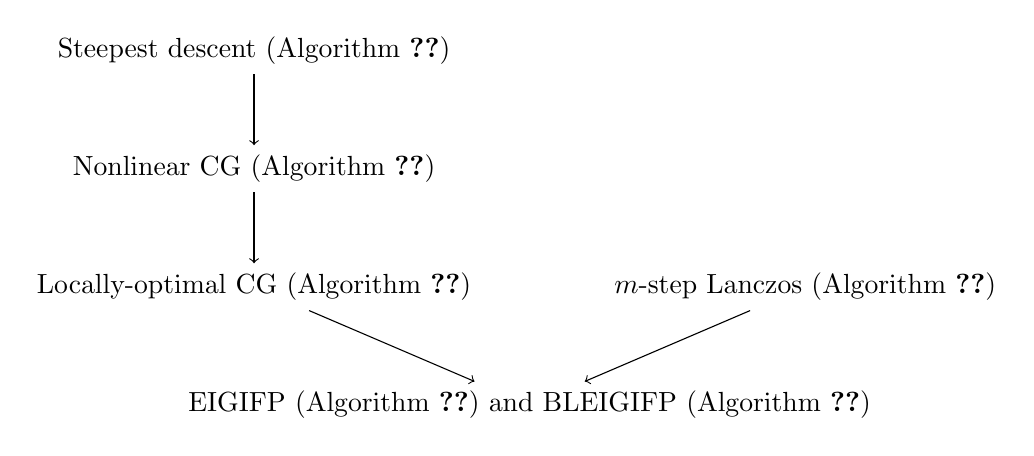
\begin{tikzpicture} 
	\node (1) at (0,4.5) {Steepest descent (Algorithm \ref{Alg:SD})};
	\node (2) at (0,3) {Nonlinear CG (Algorithm \ref{Alg:CG_nonlin})};
	\node (3) at (0,1.5) {Locally-optimal CG (Algorithm \ref{Alg:LOCG})};
	\node (4) at (7,1.5) {$m$-step Lanczos (Algorithm \ref{Alg:eigifp_inner})};
	\node (5) at (3.5,0) {EIGIFP (Algorithm \ref{Alg:eigifp}) and BLEIGIFP (Algorithm \ref{Alg:bleigifp})};
	\draw[->] (1) -- (2);
	\draw[->] (2) -- (3);
	\draw[->] (3) -- (5);
	\draw[->] (4) -- (5);
\end{tikzpicture}
\caption{Dependency chart for the EIGIFP and BLEIGIFP.}
\label{Fig:eigifp_flowchart}
\end{figure}


The Krylov subspace method underlying the EIGIFP was first introduced with a different preconditioning strategy in \cite{knyazev1987convergence}.   We consider the version proposed and analyzed in \cite{golub2002inverse} and implemented based on the technical report \cite{money2005algorithm}.  The BLEIGIFP was first presented in \cite{quillen2010block}.  For a treatment of SD and LOCG methods, the reader may reference \cite{li2015rayleigh}.





\item

We begin by developing the \textit{steepest descent} (SD) method for the GEP (\ref{Eqn:GEP}).  Recall that a steepest descent algorithm involves a function $f(x)$ which is minimized iteratively.  First, an iterate $x$ is used to determine the steepest descent direction $p$ of $f(x)$.  A linesearch is then performed to solve the problem 
\[
\min\limits_{0 < t < \infty} f(x+tp),
\]
and the solution corresponds to a new iterate $x_+$.


To develop a steepest descent algorithm for finding the smallest algebraic eigenvalue of $(A,B)$, we may frame this eigenvalue problem as the \textit{Rayleigh quotient} (RQ) minimization problem
\begin{equation}			\label{Eqn:Rayleigh_quotient_problem}
\min\limits_{x \in \bbR^n} \rho(x) := \frac{x^TAx}{x^TBx},
\end{equation}
where $\rho(x) := {x^TAx}/{x^TBx}$ is the \textit{Rayleigh quotient} (RQ), $A \in \bbR^{n \times n}$ is symmetric, and $B \in \bbR^{n \times n}$ is positive definite.  Note that we define (\ref{Eqn:Rayleigh_quotient_problem}) as a minimization problem to frame the following methods as ``descent'' method.  If $A = -A$, then (\ref{Eqn:Rayleigh_quotient_problem}) will return the largest algebraic eigenvalue of $(A,B)$.

Since $A$ and $B$ in (\ref{Eqn:Rayleigh_quotient_problem}) are real, the RQ has a well-defined gradient
\begin{equation}			\label{Eqn:Rayleigh_gradient}
\nabla \rho(x) = \frac{2}{x^TBx} \left[ Ax - \rho(x)Bx \right]
\end{equation}
and a corresponding steepest descent direction $p := -\nabla \rho(x)$.  Given an iterate $x$ of (\ref{Eqn:Rayleigh_quotient_problem}) and steepest descent direction $p$, we must now perform a linesearch by solving the problem
\begin{equation} 			\label{Eqn:Rayleigh_quotient_linesearch_general}
\min\limits_{0 < t < \infty} \rho(x+tp).
\end{equation}
If $x$ and $p$ are linearly independent, then we may perform an optimal linesearch simply by projecting the problem (\ref{Eqn:Rayleigh_quotient_linesearch_general}) onto the appropriate subspace of $\bbR^n$.  Set $t = \beta/\alpha$, $w = [\alpha; \beta]$, let $Q_1$ be a matrix with orthonormal columns spanning $\{x, p\}$, and set $A_1 = Q_1^TAQ_1$, $B_1 = Q_1^TBQ_1$.  Then we have
\begin{equation} 			\label{Eqn:Rayleigh_linesearch}
\begin{split}
\min\limits_{0 < t < \infty} \rho(x+tp)
	&	 = 			\min\limits_{0 < t < \infty}	\frac{(x+tp)^TA(x+tp)}{(x+tp)^TB(x+tp)}\cdot\frac{\alpha^2}{\alpha^2}\\
	&	 = 		\min\limits_{\alpha, \beta > 0}	\frac{(\alpha x+ \beta p)^TA(\alpha x+\beta p)}{(\alpha x+ \beta p)^TB(\alpha x+ \beta p)} \\
	&	 = 		\min\limits_{\alpha, \beta > 0}		\rho(\alpha x + \beta p)	\\
	&	 = 			\min\limits_{||w|| \neq 0} \frac{w^TA_1w}{w^TB_1w}.
\end{split}
\end{equation}
Finally, note that the steepest descent direction $p = - \nabla \rho(x)$ from (\ref{Eqn:Rayleigh_gradient}) is parallel to the GEP residual (\ref{Eqn:GEP_residual}) $r(x) = Ax - \rho(x)Bx$, and thus we may replace $p$ with $r(x)$ in (\ref{Eqn:Rayleigh_linesearch}).   Then the SD method for the RQ minimization problem (\ref{Eqn:Rayleigh_quotient_problem}) has the following sequence of steps.




\begin{algorithm}[H]
\caption{Steepest descent (SD) method for GEP}	\label{Alg:SD}

\begin{algorithmic}[1]
	\Statex		\textbf{Input:} Matrices $A, B \in \bbR^{n \times n}$ from RQ  problem (\ref{Eqn:Rayleigh_quotient_problem}), initial iterate $x_0$.
	\Statex 	\textbf{Output:} Approximate largest algebraic eigenpair $(\lambda_1, v_1)$.
	\State		\textit{Initialize:} Set $x_0 = x_0/||x_0||$, $r_0 = r(x)$ from (\ref{Eqn:GEP_residual}), $x_{-1} = 0$, $i = 0$.
	\While {not converged}
		\State	$Q_1 = \text{orth}( \{x_i, r_i \} )$.
		\State	$A_1 = Q_1^TAQ_1$, $B_1 = Q_1^TBQ_1$.
%		\State	$w_{i+1} = \text{arg}\min\limits_{||w|| \neq 0} \frac{w^TA_1w}{w^TB_1w}$.
		\State 	Find the largest algebraic eigenpair $(\rho_{i+1}, w_{i+1})$ of $(A_1, B_1)$.
		\State	$x_{i+1} = Q_1w_{i+1}$.
		\State	$r_{i+1} =r(x_{i+1})$ from (\ref{Eqn:GEP_residual}).
		\State 	$i = i + 1$.
	\EndWhile
	\State		\textit{Return:} $\lambda_1 = \rho_i$, $v_1 = x_i$.
\end{algorithmic}

\end{algorithm}



\item



While the SD method (Algorithm \ref{Alg:SD}) is computationally very simple and requires minimal memory, it can also be very slow for ill-conditioned problems, exhibiting the zig-zagging behavior typical of steepest descent algorithms.  This problem may be remedied by extending the search subspace ($Q_1$ from step 3 of Algorithm \ref{Alg:SD}) and thus modifying the search direction.  One choice for a modified search direction is to apply the \textit{nonlinear conjugate gradient} (CG) method \cite{fletcher1964function} to the RQ minimization problem (\ref{Eqn:Rayleigh_quotient_problem}), resulting in the \textit{locally-optimal conjugate gradient} (LOCG) method.  We will briefly review the linear and nonlinear CG methods in order to develop the locally-optimal linesearch strategy used in the LOCG method.



We begin with a brief summary of the \textit{linear cojugate gradient} (CG) method (for a more complete treatment, see \cite[Section 11.3]{golub2012matrix} or \cite[Chapter 5]{nocedal2006numerical}).  First developed in \cite{hestenes1952methods}, the linear CG method is a Krylov subspace method for solving the linear system $Ax = b$, where $A \in \bbR^{n \times n}$ is positive definite and the desired solution is $x_\star := A^{-1}b$.  Since $A$ is positive definite, it induces an \textit{$A$-inner product} and \textit{$A$-norm}, respectively
\begin{equation} 		\label{Eqn:conjugate_inner_product_norm}
\langle x, y \rangle_A := x^TAy, \hspace{1cm} ||x||_A := \sqrt{x^TAx}.
\end{equation}
The linear CG method generates a sequence of iterates $x_i$ which are each optimal in terms of minimizing the function 
\begin{equation}   			\label{Eqn:CG_linear_function}
\phi(x) := \frac{1}{2}||x - x_\star||_A^2 = \frac{1}{2}x^TAx + b^Tx + \frac{1}{2}b^TA^{-1}b
\end{equation}
over the Krylov subspace
\begin{equation}   			\label{Eqn:CG_linear_krylov_subspace}
\caK_i(A,q_1) = \text{span} \left\{q_1, Aq_1, \ldots, A^{i-1}q_1 \right\},
\end{equation}
where $q_1 = b$ if the initial iterate is set to $x_0 = 0$.  Note that $\phi(x)$ is convex and its gradient $\nabla \phi(x) = Ax-b$ is equal to the residual of the system $Ax=b$.  To optimize $\phi(x)$ over $\caK_i(A,b)$, a sequence of search directions $\{p_0, \ldots, p_{n-1}\}$ are created which are \textit{conjugate with respect to $A$}, meaning
\begin{equation} 				\label{Eqn:CG_conj_vectors}
p_i^TAp_j = 0 \ \ \text{for all} \ \ i \neq j.
\end{equation}


An iteration of the linear CG method has the following sequence of steps.  Given a normalized initial iterate $x_0$, the initial residual $r_0 = Ax_0 - b$ is used to create the initial search direction $p_0 = -r_0$, and we set $i=0$.  The function $\phi(x_i + t p_i)$ from (\ref{Eqn:CG_linear_function}) is minimized over $t$.  Setting $\frac{\partial}{\partial t}\phi(x_i + t p_i)$ equal to zero and solving for $t$, we find the closed-form solution
\begin{equation}				\label{Eqn:CG_linear_step_3_orig}
t_i = -\frac{p_i^Tr_i}{p_iAp_i}.
\end{equation}
Next, we update the iterate $x_{i+1} = x_i + t_i p_i$ and residual $r_{i+1} = \nabla \phi (x_{i+1}) = A x_{i+1} - b$.  Finally, we determine a new search direction $p_{i+1}$ which is conjugate to the previous set of search directions.  To satisfy this requirement, we set $p_{i+1} = -r_{i+1} + \beta_i p_i$ and require that
\[
0 = p_i^TAp_{i+1} = p_i^TA( -r_{i+1} + \beta_i p_i),
\]
giving the parameter
\begin{equation}			\label{Eqn:CG_linear_step_6_orig}
\beta_i = \frac{r_{i+1}^TAp_i}{p_iAp_i}.
\end{equation}
This sequence of steps constitutes an iteration of the linear CG method.  Yet equations (\ref{Eqn:CG_linear_step_3_orig}) and (\ref{Eqn:CG_linear_step_6_orig}) may be simplified to arrive at expressions for $t_i$ and $\beta_i$ in common literature (e.g., \cite[Algorithm 11.3.3]{golub2012matrix}, \cite[Algorithm 5.2]{nocedal2006numerical}).
To simplify (\ref{Eqn:CG_linear_step_3_orig}), assume $\beta_{-1} = 0$ and $p_{-1} = 0$.  Then for $i = 0, \ldots, n-1$ we have the search direction update $p_i = -r_i + \beta_{i-1}p_{i-1}$.  Note that $r_i$ is orthogonal to $p_{i-1}$ since $\phi(x_{i-1} + t p_{i-1})$ was minimized along $p_{i-1}$ to find $t_{i-1}$, and then we set $r_i = \nabla \phi(x_{i-1} + t_{i-1} p_{i-1})$.  Then $-p_i^Tr_i = (r_i - \beta_{i-1}p_{i-1})^Tr_i = r_i^Tr_i - \beta_{i-1}p_{i-1}^Tr_i = r_i^Tr_i $, and (\ref{Eqn:CG_linear_step_3_orig}) is equivalent to  
\begin{equation}				\label{Eqn:CG_linear_step_3_in_algo}
t_i = \frac{r_i^Tr_i}{p_iAp_i}.
\end{equation}
To simplify (\ref{Eqn:CG_linear_step_6_orig}), assume $x_0 = 0$.
By construction of the linear CG method,  each iterate $x_{i+1}$ minimizes $\phi$ over $\caK_{i+1}(A, b)$, and thus $r_{i+1} \in \caK_{i+1} (A, b)^{\perp}$.  Since $r_{i} \in \caK_{i+1}(A, b)$, we have 
\begin{equation} 		\label{Eqn:CG_linear_step_3_sub1}
r_{i+1}^Tr_i = 0 \ \ \text{for all} \ \  i = 1, \ldots, n-1.  
\end{equation}
Additionally, note that the update $r_{i+1} = Ax_{i+1} - b = A(x_{i+1} - x_i) + Ax_i - b = t_i Ap_i + r_i$ implies
\begin{equation} 				\label{Eqn:CG_linear_step_3_sub2}
Ap_i = \frac{1}{t_i}(r_{i+1} - r_i).
\end{equation}
Then the numerator in (\ref{Eqn:CG_linear_step_6_orig}) becomes
\begin{equation} 	\label{Eqn:CG_linear_step_3_sub3}
r_{i+1}^TAp_i = \frac{1}{t_i}(r_{i+1} - r_i)^T r_{i+1} = \frac{1}{t_i}r_{i+1}^Tr_{i+1},
\end{equation}
and the denominator in (\ref{Eqn:CG_linear_step_6_orig}) becomes
\begin{equation} 	\label{Eqn:CG_linear_step_3_sub4}
p_i^TAp_i = (-r_i + \beta_{i-1}p_{i-1})^TAp_i = -r_iAp_i = \frac{1}{t_i}r_i^Tr_i.
\end{equation}
And thus (\ref{Eqn:CG_linear_step_6_orig}) simplifies to
\begin{equation}			\label{Eqn:CG_linear_step_6_in_algo}
\beta_i = \frac{r_{i+1}^Tr_{i+1}}{r_i^Tr_i}.
\end{equation}



Altogether, given the steps and simplifications above, we have Algorithm \ref{Alg:CG_linear}.
\begin{algorithm}[H]
\caption{Linear conjugate gradient (CG) method}	\label{Alg:CG_linear}

\begin{algorithmic}[1]
	\Statex		\textbf{Input:} Differentiable function $\phi(x)$, initial iterate $x_0$.
	\Statex 	\textbf{Output:} Solution $x_i$.
	\State		\textit{Initialize:} Set $x_0 = x_0 / ||x_0||$, $r_0 = \nabla \phi (x_0) = Ax_0 - b$, $p_0 = -r_0$, $i = 0$.
	\While {not converged}
		\State	$t_i = \text{arg}\min\limits_{\substack{t}} \phi(x_i + t p_i) = \frac{r_i^Tr_i}{p_iAp_i}$.
		\State	$x_{i+1} = x_i + t_i p_i$.
		\State	$r_{i+1} = \nabla \phi(x_{i+1}) = Ax_{i+1} - b$.
		\State	$\beta_i = \frac{r_{i+1}^Tr_{i+1}}{r_i^Tr_i}$.
		\State	$p_{i+1} = -r_{i+1} + \beta_ip_i$.
		\State 	$i = i + 1$.
	\EndWhile
	\State		\textit{Return:} $x_i$.
\end{algorithmic}

\end{algorithm}



As a consequence of the Cayley-Hamilton theorem \cite[Chapter 12, Proposition 20]{dummit2004abstract}, the linear CG method in exact arithmetic will terminate in $n$ steps, giving $x_{n-1} = x_\star = A^{-1}b \in \caK_{n}(A,b)$ even if $\caK_{n}(A,b) \neq \bbR^n$.  
The Cayley-Hamilton theorem indicates that if $p(\lambda) = \det(\lambda I - A) = \lambda^n + a_1 \lambda^{n-1} + \cdots + a_{n-1}\lambda + a_n$ is the characteristic polynomial of $A$, then $p(A) = A^n + a_1 A^{n-1} + \cdots + a_nI = 0$.  
Then $A^{-1}p(A) = A^{n-1} + a_1 A^{n-2} + \cdots + a_{n-1}I + a_nA^{-1}$, which can be solved for $A^{-1}$ giving
\begin{equation}   	\label{Eqn:CG_linear_conv_prop_1}
x_\star = A^{-1}b =  - \frac{1}{a_n} \left( A^{n-1}b + a_1A^{n-2}b + \cdots + a_{n-1}b \right) \in \caK_{n}(A,b).
\end{equation}
Still assuming exact precision, the linear CG method has the following convergence rate
\begin{equation}		\label{Eqn:CG_linear_conv_prop_2}
\frac{||x_k - x_\star||_A}{||x_\star||_A} \leq 2  \left( \frac{\sqrt{\kappa(A)} - 1}{\sqrt{\kappa(A)} + 1} \right)^k,
\end{equation}
dependent on the condition number $\kappa (A)= \lambda_1 / \lambda_n$ \cite[Theorem 38.5]{trefethen1997numerical}.




We will now consider the \textit{nonlinear CG} method, which seeks to minimize a differentiable function $\phi(x)$.
The nonlinear CG method is nearly identical to the linear CG method (Algorithm \ref{Alg:CG_linear}) except for the absence of conjugate search directions $\{p_i\}_{i=1}^n$.
Recall the linear CG method (Algorithm \ref{Alg:CG_linear}) minimizes the convex quadratic function $\phi(x)$ defined in (\ref{Eqn:CG_linear_function}).  
If instead $\phi(x)$ is not quadratic then this function will not have a fixed positive definite Hessian, and thus any sequence of search directions $\{p_i\}_{i=1}^n$ cannot be conjugate with respect to any inner product.  
Thus the convergence properties (\ref{Eqn:CG_linear_conv_prop_1}) and (\ref{Eqn:CG_linear_conv_prop_2}) will not hold for the nonlinear CG method.  
Despite the lack of convergence guarantees, the nonlinear CG method has been well-studied, and several options exist for choosing the search direction update parameter $\beta_i$ (Algorithm \ref{Alg:CG_linear}, step 6).
The first paper to consider the nonlinear CG method \cite{fletcher1964function} used the parameter
\begin{equation}		\label{Eqn:CG_beta_nonlin1}
\beta_i = \frac{r_{i+1}^Tr_{i+1}}{r_i^Tr_i},
\end{equation} 
where $r_i = \nabla \phi(x_{i+1})$.  The author of \cite{polak1969note} found that the parameter
\begin{equation} 		\label{Eqn:CG_beta_nonlin2}
\beta_i = \frac{r_{i+1}^T(r_{i+1}-r_i)}{r_i^Tr_i}
\end{equation}
had superior performance to (\ref{Eqn:CG_beta_nonlin1}) in some cases.
Given a differentiable function $\phi(x)$ which we seek to minimize and these choices for the search direction update parameter $\beta_i$, we have Algorithm \ref{Alg:CG_nonlin}.


\begin{algorithm}[H]
\caption{Nonlinear conjugate gradient (CG) method}	\label{Alg:CG_nonlin}

\begin{algorithmic}[1]
	\Statex		\textbf{Input:} Differentiable function $\phi(x)$, initial iterate $x_0$.
	\Statex 	\textbf{Output:} Solution $x_i$.
	\State		\textit{Initialize:} Set $x_0 = x_0 / ||x_0||$, $r_0 = \nabla \phi (x_0)$, $p_0 = -r_0$, $i = 0$.
	\While {not converged}
		\State	$t_i = \text{arg}\min\limits_{\substack{t}} \phi(x_i + t p_i)$.
		\State	$x_{i+1} = x_i + t_i p_i$.
		\State	$r_{i+1} = \nabla \phi(x_{i+1})$.
		\State	\textit{Compute conjugate steplength:} $\beta_i$, e.g. (\ref{Eqn:CG_beta_nonlin1}) or (\ref{Eqn:CG_beta_nonlin2}).
		\State	$p_{i+1} = -r_{i+1} + \beta_ip_i$.
		\State 	$i = i + 1$.
	\EndWhile
	\State		\textit{Return:} $x_i$.
\end{algorithmic}

\end{algorithm}

\


xxx here

If $\phi(x) = \rho(x)$ is the Rayleigh quotient of (\ref{Eqn:Rayleigh_quotient_problem}), then the nonlinear CG method seeks to satisfy the nonlinear optimality condition 
\begin{equation}
\nabla \rho(x) = \frac{2}{x^TBx}\left[Ax - \rho(x) Bx \right] = 0.
\end{equation}


Yet when nonlinear CG is applied to the Rayleigh quotient function $\phi(x) = \rho(x)$, the update $x_{i+1}$ may be optimized over both steplengths $t_i$ and $\beta_{i-1}$.  

In the nonlinear CG method, step 4 has the form
\begin{equation}			\label{Eqn:LOCG_spans_optimal_step}
\begin{split}
x_{i+1} \ = 
	& \	x_{i} + t_{i} \left( -r_{i} + \beta_{i-1} p_{i-1} \right) \\
	\in \	&	 \ \text{span} \left\{	x_{i}, r_{i}, p_{i-1}	\right\} 		\\
	= \ 	&	 \ \text{span} \left\{	x_{i}, r_{i}, x_{i-1}	\right\}.
\end{split}
\end{equation}

xxx ABOVE USES: step 7 in Algorithm \ref{Alg:CG_nonlin}, THEN step 4 in same algo

Then if we set $Q_1 = \text{orth}([x_{i-1}, x_i, r_i])$, $A_1 = Q_1^TAQ_1$, and $B_1 = Q_1^TBQ_1$, an argument similar to (\ref{Eqn:Rayleigh_linesearch}) demonstrates that the optimal linesearch for $t_i, \beta_{i-1}$ will be the solution to the problem
\begin{equation}
\min\limits_{||w|| \neq 0} \frac{w^TA_1w}{w^T B_1 w}.
\end{equation}


\


Applying the optimal linesearch for the RQ problem, the nonlinear CG method becomes the locally-optimal conjugate gradient (LOCG) for the RQ problem.  This algorithm can also be viewed as the SD method with the addition of $x_{i-1}$ in the search space.

\begin{algorithm}[H]
\caption{Locally-optimal conjugate gradient (LOCG) for GEP}	\label{Alg:LOCG}

\begin{algorithmic}[1]
	\Statex		\textbf{Input:} Matrices $A, B \in \bbR^{n \times n}$ from RQ  problem (\ref{Eqn:Rayleigh_quotient_problem}), initial iterate $x_0$.
	\Statex 	\textbf{Output:} Approximate largest algebraic eigenpair $(\lambda_1, v_1)$.
	\State		\textit{Initialize:} Set $x_0 = x_0/||x_0||$, $r_0 = r(x_0)$ from  (\ref{Eqn:GEP_residual}), $x_{-1} = 0$, $i = 0$.
	\While {not converged}
		\State	$Q_1 = \text{orth}(\{x_{i-1}, x_i, r_i\})$.
		\State	$A_1 = Q_1^TAQ_1$, $B_1 = Q_1^TBQ_1$.
		\State	Find the largest algebraic eigenpair $(\rho_{i+1}, w_{i+1})$ of $(A_1, B_1)$.
		\State	$x_{i+1} = Q_1w_{i+1}$.
		\State	$r_{i+1} =r(x_{i+1})$ from (\ref{Eqn:GEP_residual}).
		\State 	$i = i + 1$.
	\EndWhile
	\State		\textit{Return:} $\lambda_1 = \rho_i$, $v_1 = x_i$.
\end{algorithmic}

\end{algorithm}





\item


xxx MAKE CLEAR WE JUSTIFY shift-and-invert strategy before stating algo

The inverse-free preconditioned Krylov subspace (eigifp) method extends the SD subspace $Q_1 = \text{span}\{x, (A-\rho B)x\}$ to the Krylov subspace
\begin{equation} 		\label{Eqn:eigifp_Krylov_subspace}
\caK_m(A - \rho B, x) = \text{span} \{ x, (A-\rho B)x, (A-\rho B)^2x, \ldots, (A-\rho B)^{m-1}x \}.
\end{equation}
The choice of this Krylov subspace comes from the effectiveness of shift-and-invert preconditioning strategies for solving eigenvalue problems \cite[Chapter 8]{saad2011numerical}.  To simplify notation, we briefly consider the standard eigenvalue problem.  If $\rho < \lambda_1$ is a current estimate of $\lambda_1$, then we may instead consider the shifted and inverted matrix 
\begin{equation}			\label{Eqn:shift-and-invert-SEP}
C = (A- \rho I)^{-1}.
\end{equation}
The largest algebraic eigenvalue of $C$ will have the form $\theta_1 = 1/(\lambda_1 - \rho)$, so $\rho$ and $\theta_1$ may be used to recover $\lambda_1 = \rho + 1/\theta_1$.  Additionally, if $\rho$ is close to $\lambda_1$, then $\theta_1$ will be very large and the problem of finding $\lambda_1(C)$ may be much better conditioned that the original problem $\lambda_1(A)$.  Also, if $\lambda_2 < \rho < \lambda_1$, then the shifted and inverted eigenvalue problem will have $\theta_1$ as its only positive eigenvalue.

For the GEP, the shifted and inverted matrix
\begin{equation}			\label{Eqn:shift-and-invert-GEP}
C = B(A- \rho B)^{-1}B
\end{equation}
replaces the eigenvalue problem $\lambda_1 = \lambda_1(A,B)$ with $\theta_1 = \lambda_1(C)$.  In this case
\begin{equation}
Cx = \theta_1 Bx  \ \ \ \implies \ \ \  Ax = \left( \rho + \frac{1}{\theta_1} \right) Bx,
\end{equation}
and thus  if $\rho$ is sufficiently close to $\lambda_1$ we again recover $\lambda_1 = \rho + 1/\theta_1$.

If the shift-and-invert technique is used exactly, then the shifted linear system
\begin{equation}
\left( A - \rho B \right) x_+ = Bx
\end{equation}
must be solved directly at each step.  Yet for large eigenvalue problems like the PLGD EMEP, the factorization of $A - \rho B$ is prohibitive and $C-$products must be approximated.  If we use an inverse iteration to approximate $x_+ = CBx = (A-\rho B)^{-1}Bx$, then $x_+$ will be in the subspace $\caK_m(A-\rho B, x)$ for some iterate count $m$.  Eigifp uses this ``inverse-free'' Krylov subspace, applying the corresponding projection to the shifted pencil $(A-\rho B, B)$ and updating $\rho_+ = \rho + 1/\theta_1$.  


While this is theoretically equivalent to projecting $(A,B)$ directly onto $Q_m$, the authors of \cite{golub2002inverse} observe that in practice this saves matrix multiplications by reusing $(A-\rho B)Q_m$ computed in Algorithm \ref{Alg:eigifp_inner} and is also potentially more stable (see \cite[Section 4, Example 1]{golub2002inverse}).




\item

The eigifp method has to main steps: constructing a basis for the Krylov subspace $\caK_m(A-\rho B, x)$ and solving the eigenvalue problem on this subspace to compute eigenpair updates.  Construction of the Krylov subspace is performed with Algorithm \ref{Alg:eigifp_inner}, which is computationally identical to the Arnoldi iteration if the Hessenberg matrix $H_m$ were not formed.


\begin{algorithm}[H]
\caption{$m$-step Lanczos iteration}	\label{Alg:eigifp_inner}

\begin{algorithmic}[1]
	\Statex		\textbf{Input:} Matrix $C \in \bbC^{n \times n}$, number of Lanczos steps $m$, initial approximate eigenvector $q_1$.
	\Statex 	\textbf{Output:} Basis $Q_m$.
	\State		\textit{Initialize:} Set $q_1  = q_1 / ||q_1||$, \ \ $Q_1 = [q_1]$.
	\For 			{$i = 1, \ldots, m-1$}
		\State	$z = Cq_{i}$.
		\State	$h = Q_{i}^*z$, \ \  $r_{i} = z - Q_{i}h$.
		\State	$\beta_i = ||r_i||$, \ \ $q_{i+1} = r_i / \beta_i$.
		\State	$Q_{i+1} = [Q_i \ | \ q_{i+1}]$.
	\EndFor
	\State		\textit{Return:} $Q_m$.
\end{algorithmic}

\end{algorithm}

The Lanczos iteration provides the inner iteration of the single-vector inverse-free preconditioned Krylov subspace method.  Note that step 3 of eigifp includes the previous iterate which we will label $\overline{x}$ in the search space.  This blending of the inverse-free preconditioned Krylov subspace with the CG method has been shown to accelerate the algorithm while adding minimal cost \cite{money2005algorithm}.



\begin{algorithm}[H]
\caption{Inverse-free preconditioned Krylov subspace method (eigifp)}	\label{Alg:eigifp}

\begin{algorithmic}[1]
	\Statex 	\textbf{Input:} Matrices $A, B \in \bbC^{n \times n}$ with $B$ positive definite, initial approximate eigenvector $x_0$, maximum Lanczos basis size $m$,  convergence tolerance $\textnormal{tol}_\textnormal{rel} > 0$.
	\Statex 	\textbf{Output:} Approximate largest algebraic eigenpair $(\lambda_1, v_1)$.
	\State		\textit{Initialize:} Set $x_0 = x_0/||x_0||$, $\rho_0 = x_0^*A x_0 / x_0^* B x_0$, $\overline{x} = 0$, and $i = 0$.
	\While {not converged}
		\State		\textit{Algorithm \ref{Alg:eigifp_inner}:} Perform the $m$-step Lanczos iteration on $C  = A - \rho_i B$ with initial vector $q_1 = x_i$ to obtain $Q_m$.
		\State 		Orthogonalize $\overline{x}$ against $Q_m$ to obtain $q_{m+1}$ and set $\widehat{Q}_m = [Q_m \ | \ q_{m+1}]$.
		\State		Form $A_m = \widehat{Q}_m^*(A-\rho_i B)\widehat{Q}_m$ and $B_m = \widehat{Q}_m^*B \widehat{Q}_m$.
		\State		Compute the largest algebraic eigenpair $(\theta_1, u_1)$ of $(A_m, B_m)$.
		\State		Update $\rho_{i+1} = \rho_i + \theta_1$, $x_{i+1} = \widehat{Q}_m u_1$, $\overline{x} = x_{i+1} - x_i$, and $i = i + 1$.
	\EndWhile
	\State		Set $\lambda_1 = \rho_i$, $v_1 = x_i$.
	\State		\textit{Return:} $(\lambda_1, v_1)$.
\end{algorithmic}

\end{algorithm}

If a preconditioner $L_k$ is provided at iterate $k$, then eigifp only differs in the inner Lanczos iteration.  In this case, the vector $L_kq_1$ is used to construct a Krylov subspace for the transformed eigenvalue problem $(L_k^{-1}AL_k^{-*}, L_k^{-1}BL_k^{-*})$, and then this subspace is premultiplied by $L_k^{-*}$ and orthogonalized to return $Q_m$.  For complete  implementation details, see \cite[Section 5]{golub2002inverse}.  Since the matrix $A$ in the PLGD EMEP is represented implicitly, this preconditioning is not an option.

The PLGD EMEP requires the computation of the two largest algebraic eigenvalues, yet eigifp only computes one eigenvalue at a time.  In order to compute multiple eigenvalues, eigifp is implemented with a deflation strategy.  The basic idea behind deflation is that the $k$ largest algebraic eigenvalues and eigenvectors
\begin{equation}
\Lambda_k = \text{diag}( \lambda_1, \ldots, \lambda_k), \hspace{1cm} V_k = [v_1, \ldots, v_k]
\end{equation}
are used to construct a deflated matrix
\begin{equation}
\widehat{A} = A - V_k \Lambda_k V_k^T.
\end{equation}
Passing $\widehat{A}$ to eigifp will then return $\lambda_1(\widehat{A}) = \lambda_{k+1}$.  Thus eigifp must be called $k$ times to return the $k$ largest algebraic eigenvalues.  Additionally, if these eigenvalues of $A$ are clustered, then this algorithm can converge slowly.  

The typical remedy for these challenges is to replace the single vector iterate in eigifp with a block of vectors.  The resulting block inverse-free preconditioned Krylov subspace method (bleigifp) was developed and analyzed in \cite{quillen2010block}.

\begin{algorithm}[H]
\caption{Block inverse-free preconditioned Krylov subspace method (bleigifp)}	\label{Alg:bleigifp}

\begin{algorithmic}[1]
	\Statex 	\textbf{Input:} Matrices $A, B \in \bbC^{n \times n}$ with $B$ positive definite, initial approximate eigenvectors $Q_j = [q_1, \ldots, q_j]$, maximum Lanczos basis size $m$,  convergence tolerance $\textnormal{tol}_\textnormal{rel} > 0$.
	\Statex 	\textbf{Output:} Approximate largest algebraic eigenpairs $(\Lambda_j, V_j)$.
	\State		\textit{Initialize:} For $i = 1, \ldots, j$, set $q_i = q_i/||q_i||$, $\rho_i = q_i^*A q_i / q_i^* B q_i$, and $\overline{q}_i = 0$.
	\While {not converged}
		\For {$i = 1, \ldots, j$ }
			\State		\textit{Algorithm \ref{Alg:eigifp_inner} with CG step:} Construct a basis $Q^{(i)}$ of $\{\overline{q}_i, \caK_m ( A-\rho_i B , q_i) \}$.
		\EndFor
		\State		Orthonormalize $\left\{ Q^{(1)}, \ldots, Q^{(j)} \right\}$ to obtain $Q_m$.
		\State		Form Krylov subpace problem with $A_m = Q_m^*AQ_m$ and $B_m = Q_m^*B Q_m$.
		\State		Compute the $j$ eigenpairs $(\rho_i, w_i)_{i=1}^j$ of $(A_m, B_m)$.
		\State		Update $\overline{q}_i = q_i$ and $q_i = Q_m w_i$ for $i = 1, \ldots, j$.
	\EndWhile
	\State		Set $\Lambda_j = \text{diag}(\rho_1, \ldots, \rho_j)$, $V_j = [q_1, \ldots, q_j]$.
	\State		\textit{Return:} $(\Lambda_j, V_j)$..
\end{algorithmic}

\end{algorithm}


Black-box implementations of these inverse-free preconditioned Krylov subspace methods are available in MATLAB\footnote{\url{https://www.ms.uky.edu/~qye/software.html}}.  The single-vector implementation \texttt{eigifp} is discussed in \cite{money2005algorithm}, and its block extension \texttt{bleigifp} is discussed in \cite{quillen2010block}.  In the next section, we examine the effectiveness of these methods and IRAM on the PLGD EMEP.


\end{enumerate}


